Skip to content
 This repository
Explore
Gist
Blog
Help
@kimccarty kimccarty
 
 Unwatch 5
  Unstar 1
  Fork 4
RochelleA/team_we_got_this
 branch: FinalReport  team_we_got_this/Documentation/Report/FinalReportDocuments/FinalReport/FinalReport.tex
@kimccartykimccarty 2 days ago Kim added to section 2.3 and edited everything else
1 contributor
RawBlameHistory     647 lines (506 sloc)  54.244 kb
\documentclass{article}
\usepackage[usenames,dvipsnames]{xcolor}
\usepackage{graphicx, float,amsmath, caption, subcaption}
\definecolor{DarkGray}{gray}{0.25}
\pagestyle{plain}
%opening


\begin{document}


\title{Final Report}
\author{team\_we\_got\_this}
\maketitle
\thispagestyle{plain}
\graphicspath{ {Images/} }

\tableofcontents
\listoffigures
\listoftables
\vspace{2cm}
\textcolor{red}{What are our goals? We need to be able to say in two sentence what the goal of building our simulation is? }

\pagebreak
..\section*{Introduction}
%todo	\textcolor{blue}{Describe the context for the work and the problem you are addressing. Briefly summarise what you achieved in the project.}

\section{Literature Review}
%	\textcolor{gray}{
%		\begin{itemize}
%			\item What are the possible types of traffic simulation? What are the benefits of each? 
%			\item what type of traffic simulation is in \cite{namekawa2005general}? Why is/isn't it suitable for our model?
%			\item what type of traffic simulation is used in \cite{sewall2010continuum}? why is/isn't it suitable for out model?
%			\item what have we taken from each model and why did we decide to include these attributes?
%		\end{itemize}
%	}
	
	\noindent
	In what follows we will evaluate the different traffic simulations presented in current literature. 
	We will begin by discussing the different categories of traffic simulations and their use in representing different types of road networks. 
	Thereafter we will focus on Microscopic traffic simulations as these best meet the specifications of our system presented in section \ref{RequirementsAndDeisgn}.
	
	\subsection{Background}
	
	In order to accurately study a real-life system, it is often necessary to first model this system by abstracting some information. 
	Once this model has been made, one can build a simulation to make several observations of the model. 
	Finally one analyses the information collected from the simulation in order to make inferences and suggestions \cite{sokolowski2011principles}. 
	A traffic simulation can be classified in several ways - microscopic, mesoscopic and macroscopic. 
	Another distinction of a traffic simulator is discrete or continuous. 
	In a discrete system the variables change at set intervals of time whereas in a continuous system the variables change continuously with time. 
	
	Macroscopic traffic simulations are traffic simulations capable of showing the effect of small changes on vast and complex networks. 
	Whereas a microscopic traffic simulation is used to model individual movement of cars  in smaller sections of a network. 
	For example one might use a microscopic simulation to observe movement of a vehicle in a specific intersection which has had a large number of accidents in a year. 
	Microscopic models are also more suitable for studying changes such as a new road ramp because they focus on parameters such as velocity and acceleration \cite{sokolowski2011principles}. 
	Macroscopic and mesoscopic models are similar in their approaches as they capture traffic dynamics in lesser detail. 
	This results in a faster and easier simulator which is more suitable for larger networks. 
	On the other hand, a microscopic simulator is applied to a smaller area as it better represents vehicle and driver-behaviour \cite{burghout2005hybrid}. 
	These are attributes we would like to model in our simulation, hence it would seem a microscopic model would best represent our simulation. 
	
	
	\subsection{Microscopic Simulations}
	
	Before categorising our model, it was necessary to further explore different microscopic simulations to see what other attributes we could include in our simulation.
	In \cite{namekawa2005general}, the author describes a cell automation method for realizing a microscopic model. 
	In this simulation the main aim is to have vehicles that have the capability to make their own decisions. 
	The road network has physical attributes such as widths, shapes and slopes. 
	They also have logical attributes such as traffic signals and signs. 
	A vehicle is contained within a cell, this is the state at say time $t$. 
	At the next time step, $t+1$, the vehicle will have to decide its new cell based on the information of neighbouring cells in the previous time step. 
	
	This model has many useful characteristics which we would like to implement in our traffic simulation. The first, is that by giving cells physical attributes as well as logical attributes, we could better represent different types of networks using the same simulation. 
	We could use this in our simulation to allow users to build their own road networks and specify these attributes themselves. In doing this, we hope the simulation will have a broader application. 
	The second - the use of cell automation - by recording information on neighbouring cells, cars could be modelled individually and make unique decisions based on their current position but also on any policies we introduce. 
	Cars having decision making capabilities based on their current state would also improve our ability to model more complex road structures such as roundabouts.  
	
	Another microscopic simulation that we would like to draw elements from defines a reactive agent and is presented in \cite{ehlert2001microscopic}. I
	n this paper the authors focus on intelligent agents so that vehicles can model individual driving behaviours. 
	The paper defines an intelligent agent as capable of sensing its environment and acting accordingly. This model differs from the above model as drivers can now be classed as aggressive if they break the set behaviours defined below. 
	Each agent has seven behaviours which automate its driving on the network. 
	The first, Road-following, keeps the vehicle on the road whilst the second, Intersection/Changing Lanes, ensures the driver adjusts its speed before changing its direction or reaching an intersection. 
	The Traffic Lights behaviour ensures a car stops at a red or yellow traffic light if that traffic light applies to it.  
	Another necessary behaviour implemented to simulate realistic driving is Car-following. 
	This behaviour requires that a vehicle adjust its speed if the car in front is travelling at a slower speed. 
	The behaviour, Switching Lanes, allows a car to change into another lane in order to overtake a slower car. 
	Applying Other Traffic Rules is a behaviour which allows the simulation to model other rules such as maximum speeds and one-way streets such that drivers will exhibit the necessary actions to comply with these rules. 
	Finally, the Collision Detection and Emergency Breaking behaviour alerts the car when it is about to crash into and object. 
	This behaviour takes priority over all other behaviours. 
	
	Whilst some of these behaviours are not necessary for our simpler simulation, many are crucial features which will allow our simulation to accurately measure real-life networks. 
	We would like to represent the following behaviours, as described above, in our simulation: 
	
	\begin{itemize}
		\item Road-following
		\item Traffic Lights
		\item Car-following
		\item Switching lane
	\end{itemize}
	 We have had great success in representing many of these behaviours in a few of the initial simulations we created. 
	 This will be explained in detail in section \ref{RequirementsAndDeisgn}. 
	
	
	\subsection{Conclusion}
	We believe a microscopic system will better represent our simulation because it will focus on smaller areas and individual driver capabilities. 
	We have used the different approaches presented in the two microscopic simulations to influence the requirements and implementation of our system. 
	We would like to use the cell automation used in the first simulation to control where our vehicles are at each tick of the clock. 
	In order to model a real urban environment we would like the vehicles in our system to exhibit the following behaviours, Traffic Lights, Car-following, Road-following and Switching Lanes behaviours from the second simulation.
	
%	\textcolor{red}{When we discuss the early models we made, it would be good to say tat Anton's model exhibited the Traffic lights behaviour from the paper, \cite{ehlert2001microscopic}}
%	

\section{Requirements and Design}\label{RequirementsAndDeisgn}
%	\textcolor{gray}{What did we set out to achieve?}
%todo Describe the requirements you set for your project at the
%todo beginning and the design you have taken for your project. Focus on why you decided to
%todo tackle the problem in the way you did, and what eects that had on the design. You may
%todo also wish to mention the impact of team-working on your requirements and design.

\subsection{Introduction}
	In this section we will discuss the requirements of our simulation based on the initial requirements laid out in the introductory slides, the Literature we have reviewed and based on the initial models we created. 
	We will categorise the requirements of our simulation into functional and non-functional requirements. Given this new list of requirements we will prioritise them into one of three sub-categories  --- Necessary, Optional and Extra. 
	Finally we will outline a timetable for the start and completion of each requirement.  
	
	 Software systems Requirement Engineering is an important part of software development life-cycle as it extracts the key requirements necessary to build a software. 
	 By having clear criteria, software engineers can easily analyse, implement and evaluate their system \cite{nuseibeh2000requirements}. 
	 There are five key stages of requirement engineering. The first is the elicitation of requirements where the team identifies, reviews and understands the constraints of the system. 
	 The second stage is analysing the constraints followed by writing these constraints into a requirement specification of the system. 
	 Once the specification is agreed on, the team will begin timetabling the requirements. 
	 
%	 	\subitem {\bf Requirement Elicitation}: identifying, reviewing and understanding the constraints of the system.\\
%	 	\subitem {\bf Requirement Analysis}: analysing the constraints of the system.\\
%	 	\subitem {\bf Requirement Specifcation}: clearly documenting the constraints of the system. \\
%	 	\subitem {\bf Requirement Verification}: Finalising a clear and precise agreement on the system requirements.\\
%	 	\subitem{\bf Requirement Management}: Timetabling these requirements.\\
%	 	
%	 
%	 	\subitem \emph{Requirement Elicitation}: identifying, reviewing and understanding the constraints of the system.\\
%	 	\subitem \emph{Requirement Analysis}: analysing the constraints of the system.\\
%	 	\subitem \emph{Requirement Specifcation}: clearly documenting the constraints of the system. \\
%	 	\subitem \emph{Requirement Verification}: Finalising a clear and precise agreement on the system requirements.\\
%	 	\subitem \emph{Requirement Management}: Timetabling these requirements.\\
%	 	 
%	 
%	 \begin{description}
%	 	 \item [Requirement Elicitation:] identifying, reviewing and understanding the \\ constraints of the system.
%	 	 \item  [Requirement Analysis:] analysing the constraints of the system.
%	 	 \item [Requirement Specification:] clearly documenting the constraints of the \\ system. 
%	 	 \item [Requirement Verification:] Finalising a clear and precise agreement on the system requirements.
%	 	 \item [Requirement Management:] Timetabling these requirements.
%	 \end{description}
%	 
%	 
%	 \begin{itemize}
%	 	\item \emph{Requirement Elicitation}: identifying, reviewing and understanding the constraints of the system.
%	 	\item \emph{Requirement Analysis}: analysing the constraints of the system.
%	 	\item \emph{Requirement Specifcation}: clearly documenting the constraints of the system. 
%	 	\item \emph{Requirement Verification}: Finalising a clear and precise agreement on the system requirements.
%	 	\item \emph{Requirement Management}: Timetabling these requirements.
%	 \end{itemize} 
	 
	 
\subsection{Requirement Elicitation}	
%    Following the initial requirements from the Introductory Lecture Slides, we created a list of all requirements for the simulation. We then separated them into  categories based on what was necessary, what was optional if we had time, and what would be done if we added the optional items and still had extra time. Table \ref{requirements} demonstrates the categories.


The following initial requirements come from the \textcolor{black}{\emph{Introductory Lecture Slides:}}\\\\
{\bf\textcolor{MidnightBlue}{Meta-requirements:}}
\begin{itemize}
	
	\item Development must be coordinated through github repository.
	\item The source code can be written in any language.
	\item Documentation must be provided in Latex format and exported as PDF.
	\item Unit testing of high quality and coverage should be performed.
	\item Code documentation and comments for methods and variables should be provided.
	\item Work should be critically evaluated to highlight encountered problems and also parts of the project that worked well.
\end{itemize}

{\bf\textcolor{MidnightBlue}{System Requirements:}}
\begin{enumerate}
	
	\item The system must simulate individual vehicles such as cars, coaches and buses.
	\item The road network must have different parts including roundabouts and multi-lane junctions. 
	\item The network must have places where vehicles enter and exit.
	\item The model should be able to simulate individual behaviour of drivers, e.g. reckless, cautious and normal. 
	\item The system should be able to time each car's journey to present efficiency statistics according to purpose and patterns of use. 
	\item The simulation might support emergency services such as ambulances and give them priority at traffic lights.
	\item The model should be able to make use of different policies and test their effectiveness and report on their success or failure rates using a particular measure (e.g. average speed, congestion rate).
	\item The engine should have a particular state which depends on how long the simulation has run for and a time granularity constant (macroscopic or microscopic) must be chosen which indicates on how often the state is updated, with vehicles changing their position and new cars being created, old cars being removed.  
	\item Users should have the ability to configure their own maps of an arbitrary scale. 
	\item A GUI or command line should be used to visualise maps and simulations.
\end{enumerate}

\noindent
After considering the available requirements, our team decided to go ahead and implement a number of ideas of how such requirements can be modelled. A description of each system along with an analysis of their benefits and pitfalls are discussed in the next section. 


\subsection{Requirement Analysis}
\noindent
\begin{enumerate}
	
	\item state automaton or discrete
	[screenshot] [brief description]
	\item continuous or formula-based
	[screenshot] [brief description]

\end{enumerate}

\subsubsection{Initial Designs}
As a first task we decided to let each member brainstorm a different way to complete the assignment. We would then evaluate each approach and proceed with the one that seemed the most appropriate.


	The first option we considered was using a hexagon matrix. Essentially, the matrix would work in the same way as a normal matrix with square-shaped cells, but instead our matrix would have hexagon-shaped cells. In this way each cell would still have row and column coordinates in the matrix to track the position of cars. This method would even allow us to check the adjoining cells for cars to prevent collisions. We thought the hexagon-shaped cells would allow us to better simulate a roundabout than square-shaped cells would. In the working simple model using this method, we had achieved working traffic lights. If a light was green for straight ahead only, the cars who wanted to go straight would go while the cars who wanted to turn left would stay stopped at the light. In this simple model we had not yet enabled cars to respond to other cars. Thus if a car was travelling at a faster speed than the car in front of it, it would pass through it. When attempting to implement this as a trial of the model, we decided that a hexagon matrix was an unnecessary complication.
    
    The second option we came up with also used a matrix and was based on the cell automation model \cite{namekawa2005general}. In this model each cell of a matrix is given attributes and properties. The attributes included the width, height, and type of cell whilst the properties would give information about whether or not the cell is occupied by a vehicle. The most important feature we would include in each cell was information on its neighbouring cells so that cars could make dynamic decisions about where they would go at each tick of the clock in the simulation.
    
    The third option was actually the first working simulation that the group created. In this simulation, pixels are recoloured every thirty milliseconds to show the movement of cars across the map (\textcolor{red}{see figure \ref{NurModel}}). The entry points, exit points, and changing lanes were all dependent on the size of the static map. We had this simulation working very quickly, but we questioned whether it would be dynamic enough to adapt to our growing plans without getting overly complicated. In particular, we were concerned that this approach would hold us back as we tried to develop a multi-lane roundabout where cars would need to know when to change lanes to exit. This model originally had a similar problem with collisions as mentioned in option two where faster cars would pass through slower cars. We were able to implement a level of intelligence in the cars -- faster cars could respond to a slower car in front of them by overtaking in the right lane. If, however, the cars were already in the right-hand lane, the car would merely slow down and match the slower speed of the car in front of them while keeping a safe distance.
    
    The final option we considered was a mathematical approach on a continuous model in which our map was represented by several parametric equations dependent on time (\textcolor{red}{see figure \ref{KimModel}}). In this way, each car would have its position denoted by a set of coordinates $(x,y)$. The parametric equation used to calculate the car's next position at each time step would be determined using its current position and the intended direction of travel. This solution would simplify the problem of the  multi-lane roundabout in the previous approach by merely using two sets of parametric equations for two concentric circles. Although this approach would allow us to accurately calculate where each car is at any given time, it would be difficult to come up with an efficient way to check for nearby vehicles. For this reason and other difficulties we foresaw, we decided this implementation would be unnecessarily time-consuming.  


\subsubsection{Foreseen Difficulties}

\textcolor{red}{Kim will add commentary on the changing lanes and traffic jam diagrams}

\subsubsection{[insert name]}
\textcolor{green}{\indent We planned to first build the road and get the cars to properly drive on them with a basic intersection. Our first working model was hard coded to depend on the size of the map and used traffic lights to regulate the flow of traffic. We decided to move on from this to use a grid based model in which we would add in a roundabout. The first model would need to be adapted whenever the map changed. Also a roundabout would have been difficult to implement in this way since the cars have x- and y-coordinates. Though a grid is discrete, we would attempt to make it as continuous as possible by making the squares of the grid as small as possible. We would first implement the roundabout with no traffic lights, attempt to break it by creating a heavy flow from one direction which in turn would block cars from entering at the next junction. We would then fix this problem by adding in traffic lights to regulate the flow of cars into the roundabout. We also planned to have multiple lanes leading into and out of the roundabout as well as a timer to start and let it run for a set amount of time.	
\newline\indent	If we finished with the necessary requirements of our simulation we planned to add in the requirements we designated as optional. In our research we came across a special type of roundabout called a spiral roundabout that has been implemented in northern London. In this type of roundabout a car need only to enter into the designated lane of the roundabout and it need never change lanes to exit. See figure (INSERT REF TO SP ROUNDABOUT DRAWING). One problem we foresaw with a normal roundabout was giving the intelligent to cars for when to change lanes and not cause accidents. The spiral roundabout was our solution to this problem. We also hoped to be able to implement emergency vehicles which could bypass the traffic lights and change lanes to get around cars in its way. Our last optional requirement was dynamic traffic lights which would depend on the number of cars coming from each junction into the roundabout.
\newline\indent	If both the necessary and optional requirements were implemented and there was still time to be spared, we would try to implement any of the requirements we listed as 'extra.' This included different types of vehicles such as buses, places for cars to park, a zebra crossing where cars would have to stop to wait for a pedestrian to cross if one appeared. We would also try to give the cars behavior such as differing levels of recklessness or caution as well as the ability to honk their horn at a slow driver who would then speed up as a reaction.
\newline\indent	We thought that creating categories like this would give us a step-ladder approach to first get the basics and then go for the slightly more advanced version before adding in extra elements.}

\subsection{Requirement Specification and Verification}

Given the models analysed, we can define new requirements which are more precise than elicited ones. We will begin by categorising them into functional and non-functional requirements. In table \ref{PriorityListing}, we specify the priority of each of the requirements and it is this priority list which will dictate the timetable of the project outlined in section \ref{Requirement Management}.\\

\subsubsection{Non-functional Requirements}
\textbf{Reporting:} The system should report on the results of a run simulation according to a number of factors: how conjectured the roads were (percentages of road cells occupied by cars to empty road cells) and how long it took cars to get from A to B (in respect to the minimum time it would have taken them without any other cars).\\

\noindent
\textbf{Performance / response time:} The simulation should run without lag on a regular University computer (e.g. in MSc lab 534), i.e. 64-bit Inter Core2 Quad CPU @ 2.5GHz for a medium-size simulation. 
However, when the complexity increases to more than 500x500 cells and 250 cars, the system is allowed to show a reasonable decrease in performance. 
With 1000x1000 cells and 500 cars, system is not guaranteed to continue responding to user input or show feedback on its state.\\

\noindent
\textbf{Testability:} The code for the project must be written by programmers with a fact in mind that it will have to be tested using a unit test framework. For example, when writing in Java, the unit-testing framework would be JUnit. 
Tests might be written beforehand to promote test-driven development, but it is not compulsory. 
On the other hand, it is required that every method has a corresponding test code written for it to make sure it works correctly in a variety of situations, such as boundary and corner conditions, therefore edge-cases must be tested.\\

\noindent 
\textbf{Usability:} It must be easy for users to understand how to use the simulation capabilities. Jakob Nielsen's 10 general principles for interaction design [\textcolor{red}{ref: http://www.nngroup.com/articles/ten-usability-heuristics/}] should be considered and applied for implementation of user interface, for example there should be a match between the system and real world so users understand the analogy. 
This means that cars in the simulation should look like cars and the designs for road and roundabouts must be as realistic as possible. 
Also, help should be provided for users with explanations of how to use the simulation engine. 
A heuristic testing for all the 10 principles must be performed in the end of the UI’s development life-cycle by an expert. \\

\noindent 
\textbf{Portability:} The system should be able to run on a computer with JVM installed (thus ensuring that the program can be started on any device which supports Java) or as an applet on a web-page. \\

\noindent
\textbf{Maintainability:} The code should make use of interfaces and appropriate design patterns to make sure that all programmers can understand it and make required changes (refactor it) easily.\\

\noindent 
\textbf{Extensibility:} It should be possible to introduce new features into the system without having to restructure the engine’s core if additional requirements emerge. 
For example an appropriate level of abstraction should be used to ensure that a cyclist lane occupied by cyclists, taxis, buses and motorbikes can be incorporated into the system at the later stages of development.\\

\noindent
\textbf{Documentation:} Every public method must be documented in the source code in Javadoc-style, including the purpose of the function, description of each parameter and return value, as well as clarification of exceptions using @param, @return, and @throws tags. @author and @version tags must be specified for each class. 
Documentation of a private method is encouraged when it can help other people working on the project to understand its purpose. 
Finally, UML diagrams (use-case, class and sequence at least) must be created in the design stage to make sure the principles of the overall model are clearly conveyed to shareholders and the team of developers.  

\subsubsection{Functional Requirements}
{\bf Map Designer}
\begin{enumerate}
	\item Users should be able to create a new blank map by specifying its width and height in cells. 
	\item Users should be capable to click on each cell and choose whether it is empty or a road.
	\item If a cell is a road, users should be able to specify in which direction it is going (NORTH, EAST, SOUTH or WEST).
	\item If a cell is a road, users should have an option to make it an entry node or an exit node.
	\item If a cell is a road, users can place a traffic light on it or remove an existing traffic light from it. 
	\item A map can be saved to a file with the .map extension which contains binary data of a serialised grid object.
	\item Users can load a map saved earlier by choosing a file.
    \item  Users should be able to erase all objects from the map (i.e. to start over). 
	\item Map builder should be programmed in ActionScript 3.0. 
	\textcolor{red}{[Screenshot of a blank map, and map with road, cars and traffic lights on it]}
\end{enumerate}


\noindent
{\bf Simulator Engine}
\begin{enumerate}
	
	\item  The system must be able to load a map file and initialise the appropriate state of the simulation.
	
	\item The cars must appear from entry nodes according to the flow specified as a parameter.
	\item The cars must disappear from exit nodes at every tick of a clock.
	\item The simulation controller must move cars according to their speed and direction, making sure that collisions do not occur, e.g. if a car needs to be moved to the next cell which is already occupied by another car, it will not be moved. In the future, a collision can be allowed to occur and cause a traffic jam, but this is subject to changes in requirements.
	\item The cars must be allowed to go ahead in their current direction or change direction when they reach a junction. 
	\item The appropriate methods should exist to make cars enter, follow and exit roundabouts.
	\item Traffic light's colour must change according to a certain delay associated with it by the global controller. \textcolor{red}{reconsider this:} The possible states are: RED, RED-AMBER, AMBER, GREEN. The exact behaviour of cars in these situations must be specified by a policy.
	\item Each car should have a timer which starts when it enters the map and stops when it exits. At this point, statistics are collected on the time taken for it to travel through the road network.
	\item  The simulation might be paused by the user and its state can be saved by him/her to load later. \textcolor{red}{do we need/have time for this?}
	\item The vehicles may be able to overtake each other. 
	\item  A behaviour may be added to each vehicle which determines the  speed at which they are driving and the decisions they make at traffic lights (e.g. always stop on AMBER for cautious drivers).
	\item Special vehicles may be included in the simulation such as ambulances, fire brigades and police services. These special vehicles will get priority at traffic lights and other vehicles will be required to change lanes to give way. 
	\item A time-granularity constant should be included as a global static variable so that it can be changed easily to test the behaviour of the system and give the user freedom of control. 
	\item The model should have a GUI implemented in Java Swing with menu items at the top, grid display on the left and buttons for control on the right. 
	\item The users must be able to specify policies and receive reports when the simulation ends.  
	
\end{enumerate}

\subsection{Architectural Patterns}
Whenever a team designs a system, there are many different ways to do it and even with clear specifications it can be a challenge to decide which direction is best. 
Consequently, a software architect can make use of design patterns -- the proven good design structures which have emerged from hard-won architectural knowledge \cite{bass2007software} -- to decide their approach. 
In our system, we will implement a number of design patterns to make sure we use appropriate tested solutions to save time and help us work well as a team. 


\subsubsection{Layered Pattern Solution}
Complex software systems usually require a clear separation of services so that different modules can be developed and maintained by different team members. 
We will use a layered pattern to clearly show which parts make up the whole system and assign modules to each programmer in our group. 


The layered pattern divides the software into units called layers \cite{bass2007software}. 
A layer can include a number of modules which together form a cohesive set of services. 
Layers completely partition a software system and each partition is exposed through a public interface. Furthermore, the ordering is strict, which means that layers above are allowed to use services from layers below but not the other way around, i.e. a unidirectional relations rule must be ensured among the layers. One of the disadvantages of this pattern is that the addition of new layers can add up-front costs and complexity to a system. 
However, we will design it once (at this stage) since we are not planning to add new layers to our software. Please see figure \ref{Layers} for a diagram of our layered pattern. 

\begin{figure}[H]
	\centering
	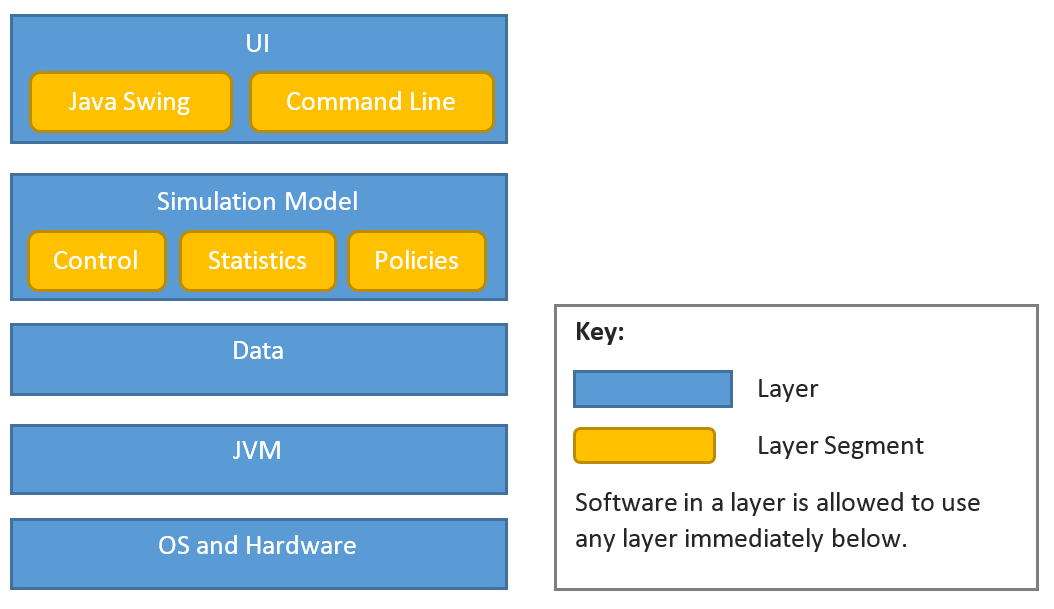
\includegraphics[width=0.7\textwidth]{Layers.png}

	\caption{Layered pattern of the simulation}
		\label{Layers}
\end{figure}

Firstly, the layered pattern diagram is a good way of providing documentation of the essential “stack” components that our system requires: an OS and appropriate hardware to run a JVM machine \textcolor{red}{[glossary]}. 
Secondly, the data layer is responsible for the handling of data from the real world, e.g. how many cars are coming from different entry points at each point in time. 
This data could be gathered from cameras installed along the roads or from the mobile apps of drivers who wish to participate in helping to gather statistics about traffic conjectures \cite{NCTA}. 
Although it would be very challenging to have our system be able to read information in a similar way, it would be \textcolor{red}{useful} to allow users to be able to specify the probability a car will enter a given junction. 
This will allow the user to correctly model their own networks and design policies to improve problems. Thirdly, the Simulation Model layer uses the provided information about cars currently using the road network and attempts to predict future states of the network. 
A number of policies will be used in a simulation and one of the aims of this project is to find the most appropriate policy by comparing their performance, thus statistics and policies are two essential sub-layers. 
The Simulation Engine will also move the cars and switch colours on the traffic lights, so control is the third sub-layer. 
Finally, the state of the model needs to be presented to the user and updated every time a change happens. 
Therefore, the final layer in our design is the UI layer, which will acquire information from the Simulation Engine layer and render it on the screen (see next section). 
Development of the GUI can take a long time because it is important for a programmer who is working on the model to see what is going on and to check if his or her code is working correctly (e.g. if a car truly changes lanes). 
Therefore, a command line output can be used which represents a road network using symbols, such as in the following example where $c$ stands for empty cell, $r$ for road and $v$ for vehicle: \\

$$
\begin{matrix}
	c & c & c & c & c \\
	r & r & v & r & r \\
	c & c & c & c & c \\
	c & c & c & c & c
\end{matrix}
$$
\\
To sum up, the Layered Pattern Solution helps us to clearly define underlying critical components of the system (OS, hardware, JVM) and create a separation of responsibilities by partitioning the system into a number of modules. 
By drawing different layers, we can see how services depend on each other and what interfaces we need to specify between them. 
Because the relations between layers is unidirectional, it is clear what parts of the system depend on each other (e.g. UI depends on the Simulation Model which depends on the data, and all three depend on the JVM).
Tasks can now be assigned to different programmers who will be working on whichever layer they prefer based on their experience and interest. 

\subsubsection{Model-View-Controller}
The second architecture pattern we will make use of is the MVC module pattern which breaks the system into three components. 
The three components are the model which represents the application's state and provides interface to application logic, the view which produces a representation of the model to the user and handles user input, and the controller which manages the interaction between the model and the view by translating user actions into changes in the model. 

\textcolor{red}{The MVC uses notifies relation to connect instances of model, view and controller}, i.e. elements are notified of a state change. 
The restrictions of this pattern are that at least one instance of each element must be created, and the model component should not interact directly with the controller. 
Finally, one of the weaknesses of the MVC design pattern is that it may introduce unnecessary complexities for simple programs \cite{bass2007software}. 
In spite of that, our system is not that simple and a number of people will be working on different parts of the simulation engine. Therefore, we decided that we will benefit from the adoption of the MVC: for example, one person will be able to work on the model (logic of moving cars according to a policy) simultaneously with another person programming the UI, such as displaying the map, importing graphics and handling user input. 

   \begin{figure}[p]
   	\centering
   	   	\begin{subfigure}{\textwidth}
   	   		\centering
   	   		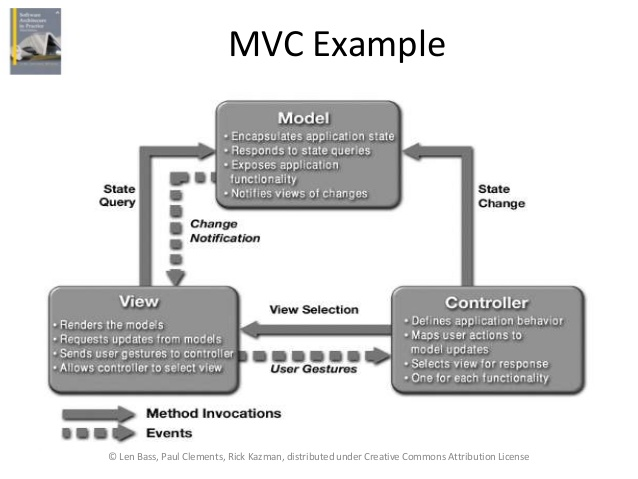
\includegraphics[width=0.75\textwidth]{MVCExample.jpg}
   	   		\caption{An example MVC structure from \cite{bass2007software}}
   	   	\end{subfigure}	
   	   	\par \bigskip
   	\begin{subfigure}{\textwidth}
   		\centering
   		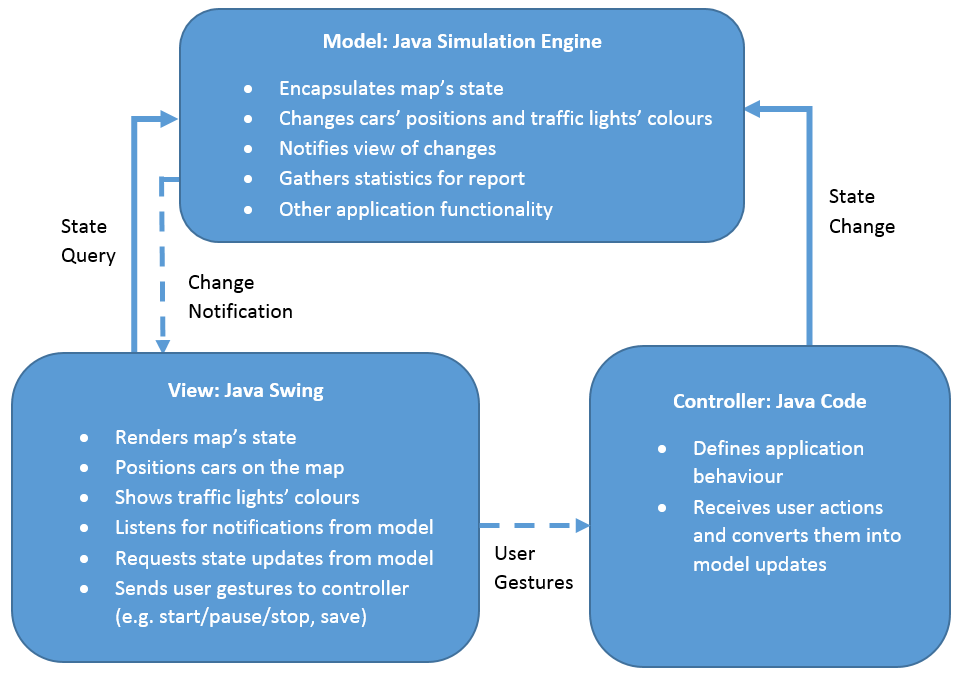
\includegraphics[width=0.75\textwidth]{mvc}
   		\caption{The MVC design for our simulation}
   		\label{OurMvc}
   	\end{subfigure}
   	

   	   \end{figure}
   	
   	\begin{figure}
   		\vspace{-35pt}
   		\centering
   		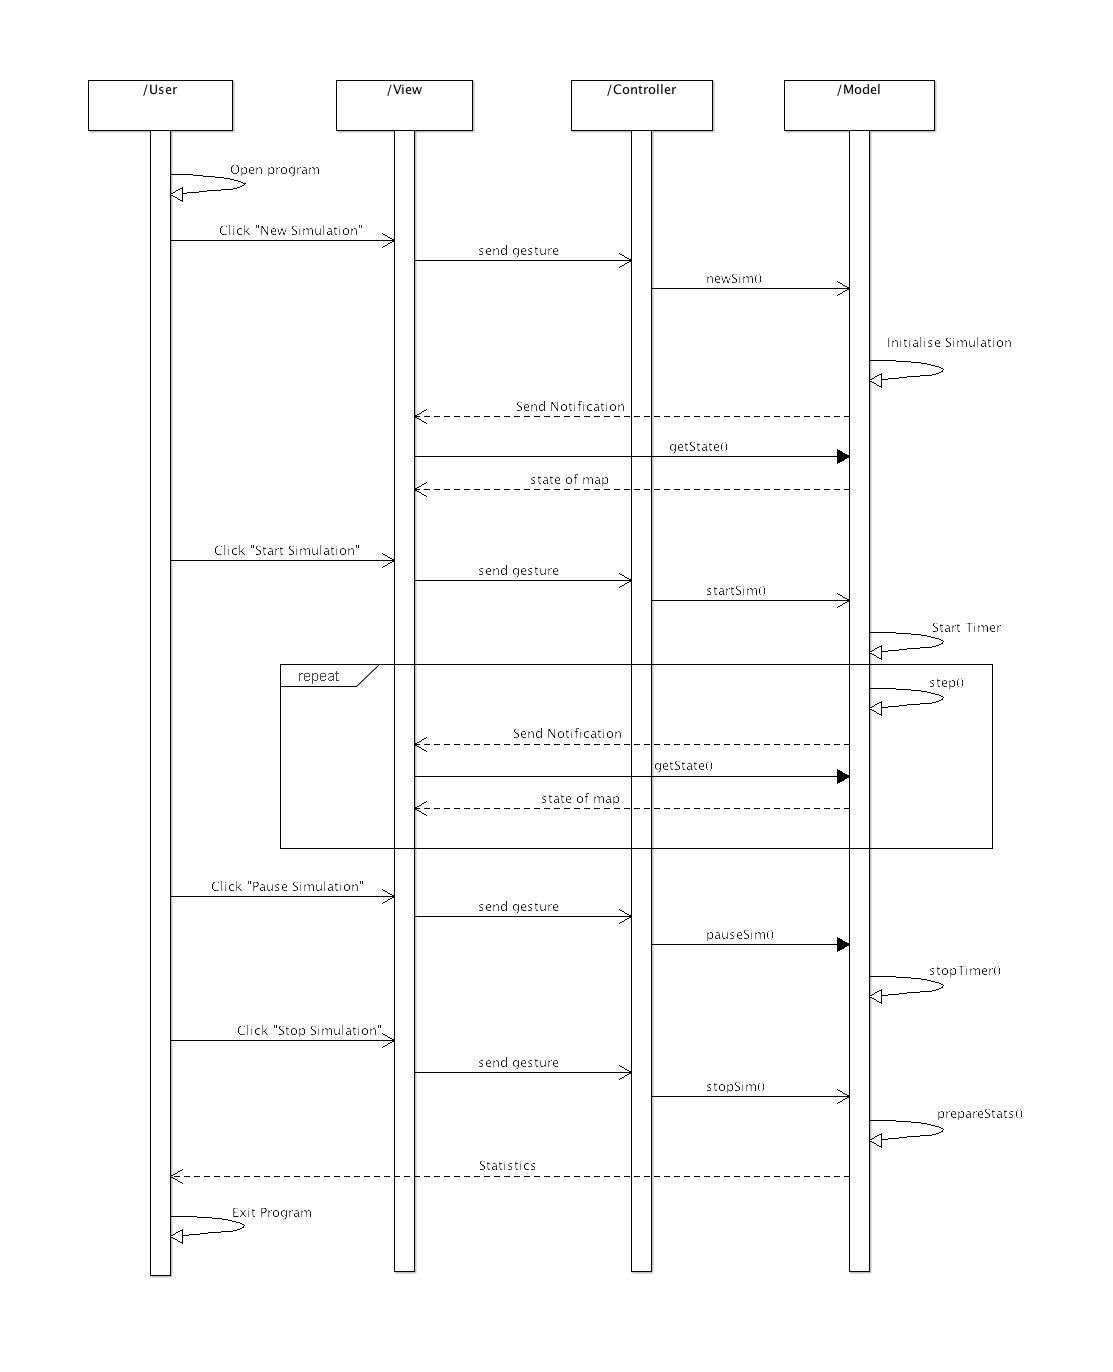
\includegraphics[width=1.15\textwidth]{SequenceDiagram}
   		\caption{The sequence diagram of an example run of the simulation}
   		\label{SequenceDiagram}
   	\end{figure}
   	

%
%\begin{figure}[h]
%	\centering
%	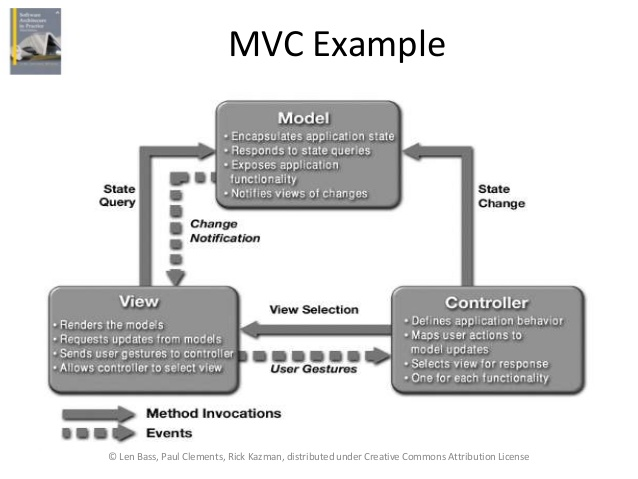
\includegraphics[width=0.7\textwidth]{MVCExample.jpg}
%	\caption{An example MVC structure from \cite{bass2007software}}
%\end{figure}

   Our MVC design differs from the design pattern in one way: the controller does not need to change between views because there is only going to be one view (the representation of the map). 
   It is allowed to deviate from the design pattern structures slightly so that it can suit the system's needs and enhance performance. 
   
   In every other way, our MVC is the same as in the design pattern: the model is responsible for running the traffic simulation, i.e. updating traffic lights, positioning cars and sending notifications of the updates to the view. Upon receiving the notification, the view queries the model and receives its state in response. 
   When the user wants to pause (start, stop, or restart) the simulation, he or she clicks on certain buttons in the GUI and the gesture is sent to the controller which translates it into an appropriate message for the model. 
   The model performs necessary transformations (e.g. going back to the initial state in case of a restart) and notifies the view about the update. 
   The overall diagram for the MVC and a sequence diagram for a typical run of a simulation are presented in diagrams \ref{OurMvc} and \ref{SequenceDiagram}. \\
   
\textcolor{red}{Problems with UML can three of them be combined on the same page to save space. Explain them here.}

\subsection{Requirement Management}\label{Requirement Management}
\textcolor{red}{How can we explain the attributes above if some have already been described in the above functional requirements\\
}

Once we defined our functional and non-functional requirements, it was clear that there were a large number of requirements. 
Although we would like to include every attribute in our system, in order to clearly manage the requirements, we needed to know in what order we should complete them. 
This would help in creating a schedule for each requirement to be completed so that we could identify which elements were dependent on the completion of another. 
For example, when building dynamic traffic lights, which would change colour based on the number of cars passing by it, we would first need traffic lights that vehicles would respond to and that would change colour based on a timer. 
Hence in our specification of the requirement we have given to each attribute a priority:\\

\noindent
\textcolor{MidnightBlue}{\bf Necessary}
- a requirement is prioritised as necessary if it is a core component of the simulation which is deemed to be necessary to achieve our original goals.\\

\noindent
\textcolor{MidnightBlue}{\bf Optional} - A requirement is categorised as optional if its inclusion would be an important benefit to the overall system but without it we will still achieve our goals.\\

\noindent
\textcolor{MidnightBlue}{\bf Extra} - A requirement is defined as extra for two reasons. 
The first is that it is an unnecessary attribute but would build a more realistic simulation. 
The second reason is that although we might feel the attribute is important it would be too time consuming to build in the given time frame.\\\\

%\begin{itemize}
%	\item \textcolor{MidnightBlue}{Necessary} - a requirement is prioritised as necessary if it is a core component of simulation which deem to be necessary to achieve our original goals. 
%	\item  \textcolor{MidnightBlue}{Optional} - a requirement is categorised as optional if it's inclusion would be an important benefit to the overall system but without it we will still achieve our goals.
%	\item \textcolor{MidnightBlue}{Extra} - a requirement is defined as extra for two reasons. The first is that it is an unnecessary attribute but would build a more realistic simulation. The second reason is that although we might feel the attribute is important it would be too time consuming to build in the given time frame.
%\end{itemize} 



\begin{table}[H] 
	\centering
	\label{PriorityListing}
	\begin{tabular}{|c|c|c|}
		\hline \rule{0pt}{2.5ex}
		\textcolor{MidnightBlue}{\bf Necessary}      & \textcolor{MidnightBlue}{\bf Optional} & \textcolor{MidnightBlue}{\bf Extra}   \\ \hline \rule{0pt}{2.5ex}
		Roads & Spiral roundabout & Buses  \\ 
		Cars & Emergency vehicles & Parking \\ 
		Roundabout & Dynamic traffic lights & Zebra crossing \\ 
		Multiple lanes & & Driver Behaviour  \\
		Traffic lights & & Horns/honking \\
		Car timer  & & \\ \hline 
	\end{tabular}
	\caption{Priority listing for the requirement of our system}
	\label{requirements}
	
\end{table}

\textcolor{red}{Add intro to section, explanation of table and Nur's Gantt diagram.}\\\\
\begin{table}[H]
	\centering
	\label{TimetableForTheProject}
\begin{tabular}{|c|c|c|c|c|}
	\hline {\bf Name} & {\bf Priority} & {\bf Start} & {\bf End} & {\bf Dependency} \\ 
	\hline 1. Road & Necessary &  &  &  \\ 
	\hline 2. Cars& Necessary &  &  &  \\ 
	\hline 3. Roundabout & Necessary &  &  & 1 \\ 
	\hline 4. Multiple Lanes & Necessary &  &  & 1 \\ 
	\hline 5. Traffic Lights & Necessary &  &  &  \\ 
	\hline 6.  Car Timer & Necessary &  &  & 2 \\ 
	\hline 7. Spiral Roundabout & Optional &  &  & 3 \\ 
	\hline 8. Emergency Vehicle & Optional &  &  & 2 \\ 
	\hline 9. Dynamic Traffic Lights & Optional &  &  & 5 \\ 
	\hline 10. Buses& Extra &  &  & 2 \\ 
	\hline  11. Parking & Extra &  &  & 1 \\ 
	\hline  12. Zebra Crossings & Extra &  &  & 1 \\ 
	\hline 13. Driver Behaviour & Extra &  &  & 2 \\ 
	\hline 14. Horns/Honking & Extra &  &  & 13 \\ 
	\hline 
\end{tabular} 
\caption{Timetable for the project}
\end{table}

\begin{figure}
	\centering
	\includegraphics[width=\textwidth]{"G Chart"}
\end{figure}

%todo	\textcolor{blue}{Describe the requirements you set for your project at the beginning and the design you have taken for your project. Focus on why you decided to tackle the problem in the way you did, and what effect that had on the design. You may also wish to mention the impact of team-working on your requirements and design.	}

\section{Implementation}
	%todo \textcolor{blue}{Describe the most significant implementation details, focusing on those where unusual or detailed solutions were required. Quote code fragments where necessary, but remember that the full source code will be included as an appendix. Explain how you tested your software (e.g. unit testing) and the extent to which you tested it. If relevant to your project, explain performance issues and how you tackle}
	In this section, we describe how we approached the implementation stage of our project. 
	We will start with the waterfall approach to implement the initial ``must'' requirements from the requirements document. This will be implemented with the help of designs such as Architectural Patterns and UML diagrams from the previous sections. We will make use of the Agile approach if we have time to include optional, non-crucial requirements such as emergency vehicles and behaviour of drivers. 
	
	
	\subsection{Project Structure}
	As defined in the design stage, our project was built around a number of components: (a) data module which simulates appearance of cars, (b) model module which is responsible for controlling the state of a grid, e.g. moving cars and changing colours of traffic lights, (c) UI to display to the user the current state of the road network, and (d) statistics to assess traffic policies. 
	For each of the following, we created a package in our project to separate responsibilities. 
	The outline and short description of each package is presented below. Finally, because we worked as a team of programmers, each person picked a package to work on, which allowed us to focus on one thing at a time and to develop ideas fully. This made sure we had a common vision of the final system which would meet the requirements and deliver the working, tested program on time. 
	
	\subsubsection{Core Package}
	The core package comprises the essential classes required for the simulation system to work. They include IGrid interface and Grid implementation, ICell and Cell, ICar and Car, ITrafficLight and TrafficLight, and others (a more detailed description can be found in the documentation section). 
	We use interfaces often to make sure our programming is not bound to concrete implementations but rather to methods provided by an interface. 
	This way a programmer working with IGrid in the View package can safely cooperate with a programmer working with IGrid in the Model package without fearing that at some point in time a method might be refactored to have a different name or do something differently than what is expected from it. 
	Furthermore, the Core package has the Program class which includes the main method to run the application.\\
	
	\noindent
	Person responsible: Anton. 

\subsubsection{Model Package}
The Model package consists of the Model class, which has a number of methods to control the state of the simulation such as change maps as a response to user input and pause, start and save simulations. 
Once a grid is loaded, the logic of changing the positions of cars and the colour of traffic lights is defined in the IGridController interface and implemented in the GridController class.\\

\noindent
Person responsible: Nur. 

\subsubsection{View Package}
The View package is maintained separately from the Model package to ensure separation of responsibilities and to abstract the business logic from representation as specified in the designs. 
It uses JFrame to create a window and JPanel to place various components on the stage, for example graphical representation of the map (GridPane), JMenu, logo and statistics graphs. 
The view depends on resources such as images of cars, empty cells and roads and updates when there is a change in the model.\\

\noindent
Person responsible: Zaki.

\subsubsection{Statistics Package}
\textcolor{red}{TODO}

\subsubsection{Events Package}
Because we are using the layered design pattern, we needed to find a way to pass messages from lower layers to higher layers. In figure 1.2, the structure is as follows: Data Layer --\textgreater Model Layer --\textgreater UI Layer. 
A common way to create messages and pass them between classes is by using an Observer pattern, the Events package contains classes and interfaces to do that: DataEvent is the object (body) of an event (e.g. a new car Event will contain coordinates of a new car in its data field), EventDispatchable is an interface which has to be implemented by a class which wants to dispatch messages and EventListener is an abstract class with methods which can be used to listen to messages.\\

\noindent
Person responsible: Anton.

\subsubsection{Test Package}
The Test package includes tests for every method in other packages written in JUnit testing framework. 
Each member of the team has to write  tests for their code as specified in the non-functional requirements specification.\\

\noindent
Person responsible: Nur, Zaki, Anton

\subsection{Setting Up a Common IDE}

Since we are using the version control system, Git, we can maintain the main remote repository in which all the code will go. 
When people make changes to the code, they commit it to the remote branch on GitHub, and others fetch it to keep an up-to-date version of the system in the local repository. 
We are also using Eclipse IDE so we can make it update the files in the project folder when a commit with changes is pulled from GitHub to the local computer.\\

\noindent
To accomplish this task, one of us creates a new project in Eclipse in the Git folder (Software/Final Model/Java\_SimulationEngine). 
Then each programmer on the team creates a folder on his local computer which will serve as his/her local Git:\\

mkdir sim\\

cd sim\\

\noindent
Then a team member initialises the Git in this folder and adds a remote origin from the SimulationEngine branch:\\

\noindent
git remote add -t SimulationEngine -f origin https://github.com/RochelleA/team\_we\_got\_this.git\\

\noindent
Finally, we download all the files which we have in the repo:\\

\noindent
git checkout SimulationEngine\\

\noindent
After these steps, the sim folder looks like this: \\
\textcolor{red}{Should we add the pics}

Final Sprint - traffic signals, statistics and UI. 

	\subsection{Documentation}
		\textcolor{gray}{export of JavaDoc, plus help for the user how to use the simulation (i.e. to start, click the start button, to finish, click stop button, etc).}
		
		
	\subsection{Testing}
%todo		\textcolor{blue}{unit testing evidence screenshots, description of typical bugs.}

\section{Team Work}
In a group project, team work plays a big part in the successes and failures of the project. In this section we discuss what roles each of the group members had and how this helped or hindered the project. We also discuss how the group handled using GitHub to work as a team and what we have learned through this experience. 

\subsection{Meetings}
 In the beginning we met twice a week to discuss the project. 
 This was a crucial part of the project and needed every team member. 
 It was here that we faced our first problems as a group. 
 There was a lack of communication which continued to be an issue for the group until the end of the project. 
 At first we struggled to find an instant message application that could be used by all members of the group. 
 For a few weeks we used a combination of both WhatsApp and text messages to communicate, but this caused issues when we would only put the message on the group WhatsApp. 
 This meant that some members of the team would not get the messages and would miss the group meetings. 
 Consequently, we needed a new form of communication and we chose Slack as an alternative which every member of the group was happy to use. 
 However, again we struggled to be consistent with our means of communication and it began to hold the group back. 
 Finally a decision was made that all important messages which needed to be read by all members of the group would be sent by KCL email as this was an application that every member had and would check frequently. 
 Although this worked well for us, it had its drawbacks. 
 The main problem was that it was not as instantaneous as an instant message and we would have to leave at least 24 hours for people to check their emails. 
 Alongside this, Rochelle, as project coordinator would send out a calendar request for all meetings so each member of the team knew when every meeting was. 
 This worked much better as no member of the group missed the team meetings as a result of not knowing they were taking place. 
 
 Another way we tried to ensure we were making the best use of our weekly meetings was to set an agenda at the start of every meeting. 
 This allowed every member of the group to bring to attention any issue they were having and also helped us to structure our meetings. 
 At the end of every meeting the project co-ordinator would create a report of the minutes of the meeting. This included the agenda, discussion point -- what was discussed in the meeting, and action points -- what each member of the team needed to do before the next meeting. 
 These reports were uploaded to GitHub so that every member could look at it if they needed to clarify anything.
 
 Once we were clear of the specifications of the system and we were ready to start designing, we gave everyone the components of the project they were to work on. Then, in the weekly meetings which were decreased to once a week, we would give feedback on what we had done. However it became clear that progress had slowed. It was decided that the waterfall model was not suited to our project and we began to follow the agile scrum method instead. \textcolor{red}{explain this method. Find a space to put the description of waterfall. Perhaps in the implementation section.}
 
 
	\subsection{Roles and Subgroups}
	
	As a team, we began by discussing what we would all like to gain from the project, where we felt we would be best used and why. 
	This allowed us to delegate roles and tasks based on what would be most advantageous to the team. 
	Whilst these roles were formed at the start of the project, throughout its duration these were adapted to meet the needs as they changed. 
	As a group we tried hard to be as flexible as possible as we realised the demands of others.
	The main roles of group members are as follows:
	
	\begin{description}
		\item [Anton] - Software engineer and architect
		\item [Kim] - Graphics coordinator
		\item [Nur] - Software engineer
		\item [Rochelle] - Project and documentation co-ordinator
		\item [Zaki] - Software engineer
	\end{description}
	
	
	\subsection{Github}
	
	In the beginning of this project our group struggled to use Github effectively because not all members of the group were familiar with it. However after the intermediate report and presentation, the group worked hard to overcome the issues we previously had with Github and since then it has become a crucial part of our software development. In this section we will discuss how we restructured our repository to better reflect how our team worked and the policies we put in place to insure members of the group could easily access the information of files they needed for their work. 
	
	Originally our team relied on a shared Dropbox folder to store our files and it was structured so every member of the group had their own sub-folder to store anything they were working on. When we began using Github, we mirrored this structure in our repository and only used a master branch. At this time any member of the group who wanted to add something to the repository would make a pull request and the project coordinator would have to approve these changes. Consequently, this approach was restrictive and unnecessarily dependant on one member. During the restructuring of the repository the project coordinator added all the other team members as collaborators. This allowed them to make changes to the repository without the coordinator approval. At this point it was necessary to add another layer of protection to repository. We opened branches for each member of the group to use to store anything they were working on. Then when they completed their work they would merge their branch with the master branch. This new policy was implemented for a brief amount of time because it also restricted the groups team work. As the software developers needed to work on the same files or make use of each others files, it impractical to have these files stored on separate branches. The group decided that the best approach for our repository was to have branches based on the features of our simulation. 
	
	Consequently, there are four main branches used in our repository. The first is the \emph{simulation engine} which is the branch in which anyone working on the simulation layer or UI layer of system. The second branch is the \emph{map editor} branch where any files relating the the map building portion of our system our developed. The third branch we make use of in our repository is the final report branch, in which all files associated to the \emph{final report} stored. This was a useful branch for our team because although not all members of the group were working on the report, they needed to have access to it in order to make sessions on what they would like to have included in it.  The final branch in our repository is the \emph{master} and this branch is only allowed to store finished work. 
	
\section{Evaluation}
%todo	\textcolor{blue}{Critically evaluate your project: what worked well, and what didn't? 	how did you do relative to your plan? what changes were the result of improved thinking and what changes were forced upon you? how did your team work together? etc. 	Note that you need to show that you understand the weaknesses in your work as well as its strengths. You may wish to identify relevant future work that could be done on your project}
	
	
\section{Peer Assessment}
\begin{tabular}{|c|c|}
	\hline Name & Points \\ 
	\hline Anton &  \\ 
	\hline Kimberly &  \\ 
	\hline Nur &  \\ 
	\hline Rochelle &  \\ 
	\hline  Zaki &  \\ 
	\hline 
\end{tabular} 
	
\bibliographystyle{apalike}
\bibliography{references}


\end{document}
Status API Training Shop Blog About
© 2015 GitHub, Inc. Terms Privacy Security Contact
